\section{实验} \label{exp}
%In this section, We first compare DIN with other methods including Wide\&Deep\cite{widedeep}, PNN\cite{PNN}, deepFM\cite{DeepFM} and Logistic Regression on two public dataset. DINs need to be evaluated on dataset with user behaviors, but not all dataset about CTR prediction contains user behaviors. Two public datasets with user behaviors: Amazon Dataset\footnote{http://jmcauley.ucsd.edu/data/amazon/} and MovieLens\footnote{https://grouplens.org/datasets/movielens/20m/} are used in this paper. Then our proposed methods are evaluated on Alibaba product data. We evaluate the effectiveness of the proposed structure of Deep Interest Network, activation function: Dice as well as the Mini-batch Aware Regularization Technique.

%In this section, we conduct empirical study on the performance of proposed DIN model and training techniques.
本节详细介绍实验，包括数据集、评价指标、实验设置、模型比较以及相应分析。
在两个包含用户行为的公开数据集以及从阿里巴巴展示广告系统采集的数据集上的实验表明，所提方法有效，并且在 CTR 预测任务上优于 SOTA 方法。
公开数据集和实验代码均已开放\textsuperscript{\ref{code}}。%\footnote{Experiment codes on two public datasets are available at GitHub: https://github.com/zhougr1993/DeepInterestNetwork}.

\subsection{数据集与实验设置}
\textbf{Amazon Dataset\footnote{http://jmcauley.ucsd.edu/data/amazon/}.}
Amazon Dataset 包含来自 Amazon 的商品评论和元数据，被用作基准数据集\cite{Amazon:AUC,AmazonData,ICCV_Amazon}。我们在名为 Electronics 的子集上进行实验，该子集包含 192,403 个用户、63,001 个商品、801 个类别和 1,689,188 个样本。该数据集中的用户行为较为丰富，每个用户和商品都有超过 5 条评论。特征包括 goods\_id、cate\_id、用户评论过的 goods\_id\_list 和 cate\_id\_list。设某个用户的全部行为为 ($b_1, b_2, \ldots, b_k, \ldots, b_n$)，任务是利用前 k 个评论过的商品预测第 (k+1) 个评论商品。
    对每个用户，使用 $k = 1, 2, \ldots, n - 2$ 生成训练数据集。在测试集中，我们给定前 $n-1$ 个评论商品来预测最后一个。
    对所有模型，我们使用带指数衰减的 SGD 作为优化器，其中学习率从 1 开始，衰减率设为 0.1。%We also tried Adam\cite{Adam}, which provides faster convergency but brings worse results than SGD for all deep models.
    mini-batch 大小设为 $32$。

    
\textbf{MovieLens Dataset\footnote{https://grouplens.org/datasets/movielens/20m/}.} MovieLens 数据\cite{MovieLens} 包含 138,493 个用户、27,278 部电影、21 个类别和 20,000,263 个样本。为了使其适用于 CTR 预测任务，我们将其转换为二分类数据。原始用户电影评分是 0 到 5 之间的连续值。我们将评分为 4 和 5 的样本标记为正样本，其余标记为负样本。我们根据 userID 将数据划分为训练数据集和测试数据集。在全部 138,493 个用户中，随机选择 100,000 个进入训练集，约 14,470,000 个样本，其余 38,493 个进入测试集，约 5,530,000 个样本。任务是基于历史行为预测用户是否会给定某部电影超过 3 分，即正标签。特征包括 movie\_id、movie\_cate\_id 以及用户评分过的 movie\_id\_list、movie\_cate\_id\_list。我们使用与 Amazon Dataset 相同的优化器、学习率和 mini-batch 大小。

\textbf{Alibaba Dataset.} 我们从阿里巴巴在线展示广告系统采集流量日志，其中两周的样本用于训练，随后一天的样本用于测试。训练集和测试集大小分别约为 20 亿和 1.4 亿。对于所有深度模型，全部 16 组特征的 embedding 向量维度均为 12。%So the input dimension of first layer in MLP is 192.
MLP 层设置为 $192 \times 200 \times 80 \times 2$。由于数据规模巨大，我们将 mini-batch 大小设为 5000，并使用 Adam\cite{Adam} 作为优化器。我们采用指数衰减，其中学习率从 0.001 开始，衰减率设为 0.9。

上述所有数据集的统计信息如表 \ref{table:Statistics} 所示。
Alibaba Dataset 的规模远大于 Amazon 和 MovieLens，因此带来了更多挑战。

    
\begin{table}[!t]
%\setlength{\belowcaptionskip}{-1cm}
\caption{本文使用的数据集统计。}
\small
\centering
\begin{threeparttable}
\begin{tabular}{lcccc}
\toprule
    Dataset       & Users & Goods\tnote{a} & Categories & Samples \\ \midrule
Amazon(Electro). & 192,403 & 63,001 & 801 & 1,689,188 \\ 
MovieLens. & 138,493 & 27,278 & 21 & 20,000,263 \\
Alibaba.  & 60 million & 0.6 billion & 100,000 & 2.14 billion \\ 
\bottomrule
\end{tabular}
\begin{tablenotes}%[para,flushleft]
        \item[a] 对于 MovieLens 数据集，商品指电影。
        %\item[2] For security reasons we can only give an approximate number.
      \end{tablenotes}
      \end{threeparttable}
\label{table:Statistics}
\end{table}    




\begin{figure*}[!t]
\centering

\includegraphics[height=6.2in, width=6.2in, keepaspectratio]{images/exp/reg_new.png}
\caption{Alibaba Dataset 上使用不同正则化的 BaseModel 性能。使用细粒度 $goods\_ids$ 特征且不加正则化进行训练时，第一个 epoch 后会出现严重过拟合。所有正则化方法都带来提升，其中我们提出的 mini-batch aware 正则化表现最好。此外，经过良好训练且使用 $goods\_ids$ 特征的模型，比不使用这些特征的模型获得更高 AUC。这来自细粒度特征中包含的更丰富信息。}
\label{fig:adaptive_reg}
\end{figure*}






\subsection{对比方法}
\label{competitors}
\begin{itemize}
\item \textbf{LR\cite{ftrl}}. 逻辑回归 (LR) 是深度网络之前在 CTR 预测任务中广泛使用的浅层模型。我们将其实现为弱基线。
\item \textbf{BaseModel}. 如第 \ref{sec:basemodel} 节所述，BaseModel 遵循 Embedding\&MLP 架构，是多数后续 CTR 建模深度网络的基础。它作为模型比较中的强基线。
\item \textbf{Wide\&Deep\cite{widedeep}}. 
在真实工业应用中，Wide\&Deep 模型已被广泛接受。
它由两部分组成：i) wide 模型，用于处理人工设计的交叉乘积特征；ii) deep 模型，用于自动提取特征之间的非线性关系，等价于 BaseModel。
Wide\&Deep 需要对 ``wide'' 模块的输入进行专家特征工程。
我们遵循 \cite{DeepFM} 中的做法，将用户行为和候选项的交叉乘积作为 wide 输入。
例如，在 MovieLens 数据集中，它指用户评分过的电影与候选电影的交叉乘积。
\item \textbf{PNN\cite{PNN}.} PNN 可以看作 BaseModel 的改进版本，它在 embedding 层之后引入 product 层，以捕获高阶特征交互。
\item \textbf{DeepFM\cite{DeepFM}}. 它将因子分解机作为 Wide\&Deep 中的 ``wide'' 模块，从而节省特征工程工作。
\end{itemize}
\subsection{评价指标}
\label{metric}
在 CTR 预测领域，AUC 是广泛使用的指标\cite{fawcett:roc}。
它通过按预测 CTR 对所有广告排序来衡量排序质量，包括用户内和用户间排序。
文献 \cite{Amazon:AUC,zhu2017optimized} 引入了一种用户加权 AUC 变体，它通过在用户上平均 AUC 来衡量用户内排序质量，并被证明与展示广告系统中的在线性能更相关。
我们在实验中采用该指标。为简洁起见，仍将其称为 AUC。
其计算方式如下：
\begin{small}
\begin{equation} \label{imps-guac}
\text{AUC} = \frac{\sum_{i=1}^{n} \#impression_i \times \text{AUC}_{i}}{\sum_{i=1}^{n} \#impression_i},
\end{equation}
\end{small}
其中 $n$ 是用户数量，$\#impression_i$ 和 $\text{AUC}_i$ 分别是第 $i$ 个用户对应的曝光次数和 AUC。

此外，我们遵循 \cite{yan2014coupled} 引入 RelaImpr 指标，用于衡量模型的相对提升。对于随机猜测器，AUC 值为 $0.5$。因此 RelaImpr 定义如下：
\begin{small}
\begin{equation}
RelaImpr = \left(\frac{\text{AUC(measured model)} -0.5}{\text{AUC(base model)} - 0.5} - 1\right) \times 100\%.
\end{equation}
\end{small}



\begin{table}[!t]
%\setlength{\belowcaptionskip}{-1cm}
\caption{Amazon Dataset 和 MovieLens Dataset 上的模型比较。所有行分别在各数据集上以 BaseModel 为基准计算 RelaImpr。}
\centering
\begin{threeparttable}
\begin{tabular}{lcccc}
\toprule
\multirow{2}{*}{Model}  & \multicolumn{2}{c}{MovieLens.} & \multicolumn{2}{c}{Amazon(Electro).}  \\ 
& AUC & RelaImpr & AUC & RelaImpr \\ \midrule
LR  & 0.7263 & -1.61\% & 0.7742 & -24.34\%  \\
BaseModel & 0.7300 & 0.00\% & 0.8624 & 0.00\%  \\
Wide\&Deep & 0.7304 & 0.17\% & 0.8637 & 0.36\%  \\
PNN  & 0.7321 & 0.91\% & 0.8679 & 1.52\%  \\
DeepFM  & 0.7324 & 1.04\% & 0.8683 & 1.63\% \\
\textbf{DIN} & \textbf{0.7337} & \textbf{1.61\%} & \textbf{0.8818} & \textbf{5.35}\%\\
\textbf{DIN with Dice}\tnote{a} & \textbf{0.7348} & \textbf{2.09\%} & \textbf{0.8871} & \textbf{6.82\%} \\ \bottomrule
\end{tabular}
\begin{tablenotes}%[para,flushleft]
        \item[a] 除 LR 外，其他行均使用 PReLU 作为激活函数。
      \end{tablenotes}
      \end{threeparttable}
\label{table:exptablePublic}
\end{table}
\vspace*{-0.4cm}





\subsection{Amazon Dataset 和 MovieLens Dataset 上的模型比较结果}
表 \ref{table:exptablePublic} 展示了 Amazon 数据集和 MovieLens 数据集上的结果。
%All the experiments are repeated 5 times with different seed, and the influence of random initialization on AUC is less than 0.0002.
所有实验重复 5 次，并报告平均结果。随机初始化对 AUC 的影响小于 0.0002。
显然，所有深度网络都显著优于 LR 模型，这确实展示了深度学习的能力。
具有专门设计结构的 PNN 和 DeepFM 比 Wide\&Deep 表现更好。
DIN 在所有对比方法中表现最佳。
特别是在具有丰富用户行为的 Amazon Dataset 上，DIN 的优势非常明显。
我们将这一结果归因于 DIN 中局部激活单元结构的设计。
DIN 通过软搜索用户行为中与候选广告相关的部分，关注局部相关的用户兴趣。借助这一机制，DIN 获得了自适应变化的用户兴趣表征，相比其他深度网络显著提升了模型表达能力。
此外，DIN with Dice 相比 DIN 进一步提升，验证了所提出的数据自适应激活函数 Dice 的有效性。




\begin{table}[!t]
%\setlength{\belowcaptionskip}{-1cm}
\caption{Alibaba Dataset 上 BaseModel 使用不同正则化的最佳 AUC，对应图 \ref{fig:adaptive_reg}。其他所有行均与第一行比较来计算 RelaImpr。}
\small
\centering
\begin{threeparttable}
\begin{tabular}{p{5cm} p{0.6cm}<{\centering} p{0.8cm}<{\centering}}
\toprule
 Regularization    & AUC  &RelaImpr \\ \midrule
Without goods\_ids feature and Reg. & 0.5940 & 0.00\% \\
With goods\_ids feature without Reg. & 0.5959  & 2.02\% \\
With goods\_ids feature and Dropout Reg. & 0.5970  & 3.19\%  \\
With goods\_ids feature and Filter Reg.  & 0.5983& 4.57\%  \\
With goods\_ids feature and Difacto Reg.  & 0.5954 & 1.49\%  \\
\textbf{With goods\_ids feature and MBA. Reg.}  & \textbf{0.6031}  & \textbf{9.68\%}  \\ \bottomrule
\end{tabular}
\end{threeparttable}
\label{table:expreg}
\end{table}



\subsection{正则化性能}
\label{sec:reg}
由于 Amazon Dataset 和 MovieLens Dataset 中的特征维度都不高（约 10 万），
包括我们提出的 DIN 在内的所有深度模型都没有遇到严重的过拟合问题。
然而，当面对来自在线广告系统且包含更高维稀疏特征的 Alibaba 数据集时，过拟合成为一项重大挑战。
例如，当使用细粒度特征训练深度模型时，如表 \ref{table_feature_set} 中维度为 6 亿的 $goods\_ids$ 特征，如果不使用任何正则化，第一个 epoch 后会出现严重过拟合，导致模型性能迅速下降，如图 \ref{fig:adaptive_reg} 中的深绿色曲线所示。
因此，我们进行了细致实验，检查几种常用正则化方法的性能。
%Here we compare several commonly used regularizations.
\begin{itemize}
\item \textbf{Dropout\cite{dropout}}. 随机丢弃每个样本中 $50\%$ 的特征 id。
\item \textbf{Filter}. 按样本中的出现频率过滤访问过的 $goods\_id$，只保留最频繁的 id。在我们的设置中，保留前 2000 万个 $goods\_ids$。
\item \textbf{DiFacto\cite{difacto} 中的正则化}. 与高频特征相关的参数受到较弱的过正则化。
\item \textbf{MBA}. 我们提出的 \textbf{M}ini-\textbf{B}atch \textbf{A}ware 正则化方法，见式 \ref{eq:batch}。DiFacto 和 MBA 的正则化参数 $\lambda$ 均通过搜索设为 $0.01$。
\end{itemize}



图 \ref{fig:adaptive_reg} 和表 \ref{table:expreg} 给出了比较结果。
观察图 \ref{fig:adaptive_reg} 的细节可以看到，与不使用细粒度 $goods\_ids$ 特征相比，使用这些特征训练的模型在第一个 epoch 中显著提升了测试 AUC 性能。
然而，在没有正则化的训练情况下，过拟合会迅速发生，见深绿色曲线。
Dropout 防止了快速过拟合，但导致收敛变慢。
频率过滤在一定程度上缓解了过拟合。
DiFacto 中的正则化对高频 $goods\_id$ 设置更大惩罚，其表现差于频率过滤。
我们提出的 mini-batch aware (MBA) 正则化相比其他所有方法表现最佳，并显著防止过拟合。

此外，经过良好训练且使用 $goods\_ids$ 特征的模型，比不使用这些特征的模型表现出更好的 AUC 性能。这是因为细粒度特征包含更丰富的信息。
考虑到这一点，尽管频率过滤略优于 dropout，但它丢弃了大多数低频 id，可能会限制模型更好使用细粒度特征的空间。


\subsection{Alibaba Dataset 上的模型比较结果}
表 \ref{table:ali} 展示了 Alibaba 数据集上的实验结果，其中使用了表 \ref{table_feature_set} 所示的完整特征集。
如预期，LR 被证明显著弱于深度模型。
在深度模型之间进行比较，我们得到若干结论。
首先，在相同激活函数和正则化条件下，DIN 本身相比所有其他深度网络，包括 BaseModel、Wide\&Deep、PNN 和 DeepFM，已经取得了更优性能。DIN 相比 BaseModel 获得了 0.0059 的绝对 AUC 提升和 $6.08\%$ RelaImpr。这再次验证了局部激活单元结构设计的有效性。
其次，基于 DIN 的消融研究证明了我们提出的训练技术的有效性。使用 mini-batch aware 正则化器训练 DIN，相比 dropout 额外带来 0.0031 的绝对 AUC 提升。此外，DIN with Dice 相比 PReLU 额外带来 0.0015 的绝对 AUC 提升。
%In all, training DIN with the two proposed techniques together brings total 0.0054 AUC gain. 

综合来看，使用 MBA 正则化和 Dice 的 DIN 相比 BaseModel 总共获得 $11.65\%$ RelaImpr 和 0.0113 的绝对 AUC 提升。即使与该数据集上表现最好的对比方法 DeepFM 相比，DIN 仍获得 0.009 的绝对 AUC 提升。
值得注意的是，在具有数亿流量的商业广告系统中，0.001 的绝对 AUC 提升在经验上已经很显著，并值得模型部署。
DIN 在更好理解和使用用户行为数据特征方面表现出明显优势。
此外，所提出的两项技术进一步提升了模型性能，并为训练大规模工业级深度网络提供了有力帮助。

\begin{table}[!t]
%\setlength{\belowcaptionskip}{-0.5cm}
\caption{使用完整特征集时 Alibaba Dataset 上的模型比较。所有行均以 BaseModel 为基准计算 RelaImpr。
DIN 显著优于所有其他对比方法。此外，使用我们提出的 mini-batch aware 正则化器和 Dice 激活函数训练 DIN 会带来进一步提升。}
\small
\centering
\begin{threeparttable}
\begin{tabular}{p{4cm} p{1.5cm}<{\centering} p{1.5cm}<{\centering}}
\toprule
Model & AUC & RelaImpr \\ \midrule
LR                                  & 0.5738 &  - 23.92\%  \\    
BaseModel\tnote{a,b}               & 0.5970 &  0.00\% \\
Wide\&Deep\tnote{a,b}               & 0.5977 &  0.72\%  \\
PNN\tnote{a,b}                      & 0.5983 &  1.34\%  \\
DeepFM\tnote{a,b}                   & 0.5993 &  2.37\%  \\
\textbf{DIN Model\tnote{a,b}}       & \textbf{0.6029} & \textbf{6.08\%} \\
\textbf{DIN with MBA Reg.\tnote{a}} & \textbf{0.6060} &  \textbf{9.28}\%  \\
\textbf{DIN with Dice \tnote{b}}    & \textbf{0.6044} &  \textbf{7.63}\%  \\
\textbf{DIN with MBA Reg. and Dice} & \textbf{0.6083} &  \textbf{11.65\%}  \\ \bottomrule
\end{tabular}
\begin{tablenotes}%[para,flushleft]
        \item[a] 这些行使用 PReLU 作为激活函数进行训练。
        \item[b] 这些行使用 dropout 正则化进行训练。
      \end{tablenotes}
      \end{threeparttable}
\label{table:ali}
\end{table}


\subsection{在线 A/B 测试结果}
2017 年 5 月至 2017 年 6 月，我们在阿里巴巴展示广告系统中进行了谨慎的在线 A/B 测试。
在近一个月的测试期间，与所介绍的 BaseModel，也就是上一版本在线服务模型相比，使用所提正则化器和激活函数训练的 DIN 带来了最高 10.0\% 的 CTR 提升和 3.8\% 的 RPM (Revenue Per Mille) 提升\footnote{在我们的真实广告系统中，广告按照 $\textsl{CTR}^\alpha \cdot \textsl{bid-price}$ 排序，其中 $\alpha > 1.0$，用于控制 CTR 和 RPM 提升之间的平衡。}。这是显著提升，并证明了所提方法的有效性。目前 DIN 已经在线部署并服务主流量。

值得一提的是，工业级深度网络的在线服务并不容易，因为每天有数亿用户访问我们的系统。更困难的是，在流量高峰时，我们的系统每秒服务超过 100 万用户。系统需要以高吞吐和低延迟进行实时 CTR 预测。例如，在真实系统中，我们需要在小于 10 毫秒内为每位访问者预测数百个广告。
在实践中，我们部署了若干重要技术，以在 CPU-GPU 架构下加速工业级深度网络的在线服务：
i) \textsl{request batching}，合并来自 CPU 的相邻请求以发挥 GPU 算力，
ii) \textsl{GPU memory optimization}，改进访问模式以减少 GPU 内存中的无效事务，
iii) \textsl{concurrent kernel computation}，允许使用多个 CUDA kernel 并发处理矩阵计算。
总体而言，这些技术的优化在实践中使单机 QPS (Query Per Second) 能力翻倍。
DIN 的在线服务也从中受益。


\subsection{DIN 可视化}
\label{visual_din}
最后，我们在 Alibaba 数据集上进行案例研究，以揭示 DIN 的内部结构。
%DIN designs the activation unit to locally activate the related behaviors with respect to candidate ads. 
我们首先考察局部激活单元的有效性。
图 \ref{fig:att_case} 展示了用户行为相对于候选广告的激活强度。
正如预期，与候选广告高度相关的行为获得了较高权重。


%\begin{figure*}[!h]
\begin{figure}[!ht]
\centering
%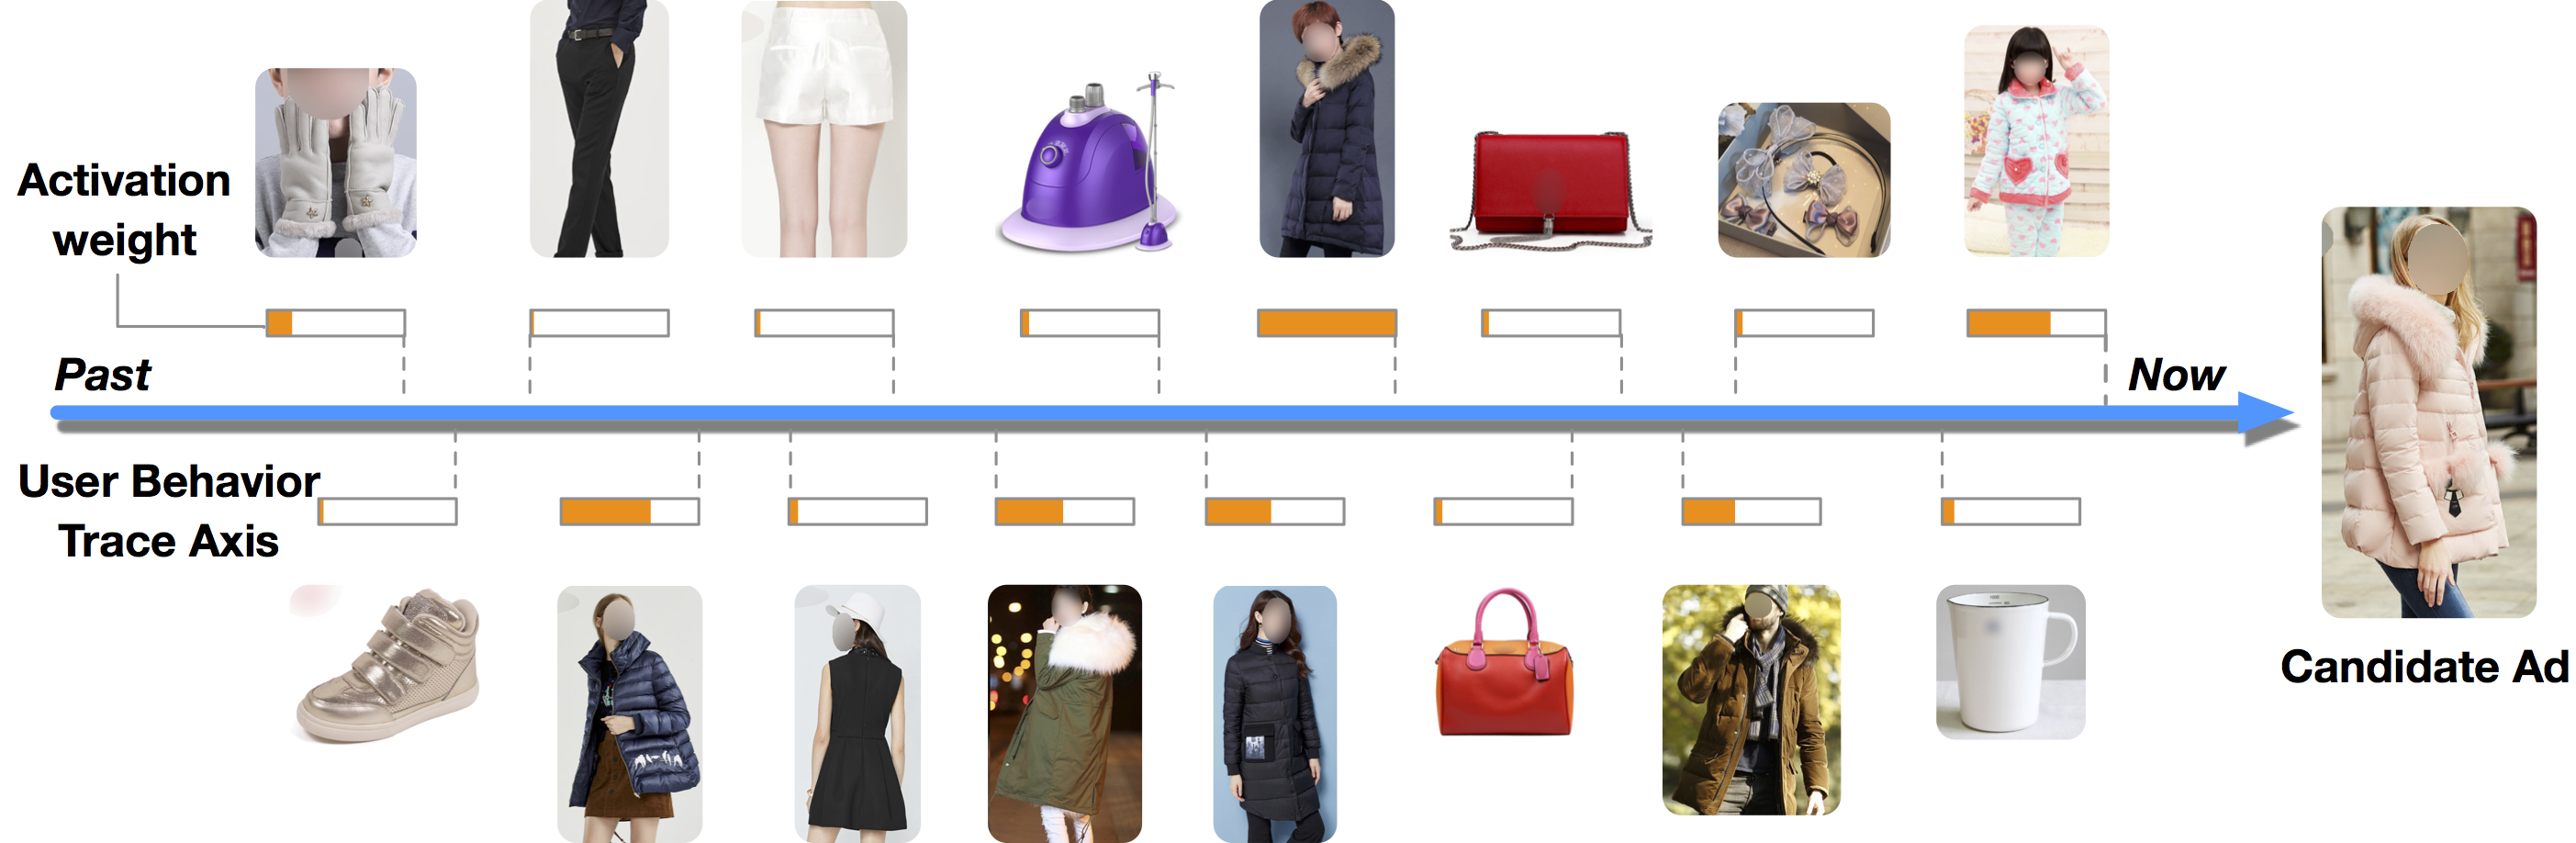
\includegraphics[height=3.5in, width=5in, keepaspectratio]{images/omni/attention_timeline_fix.pdf}
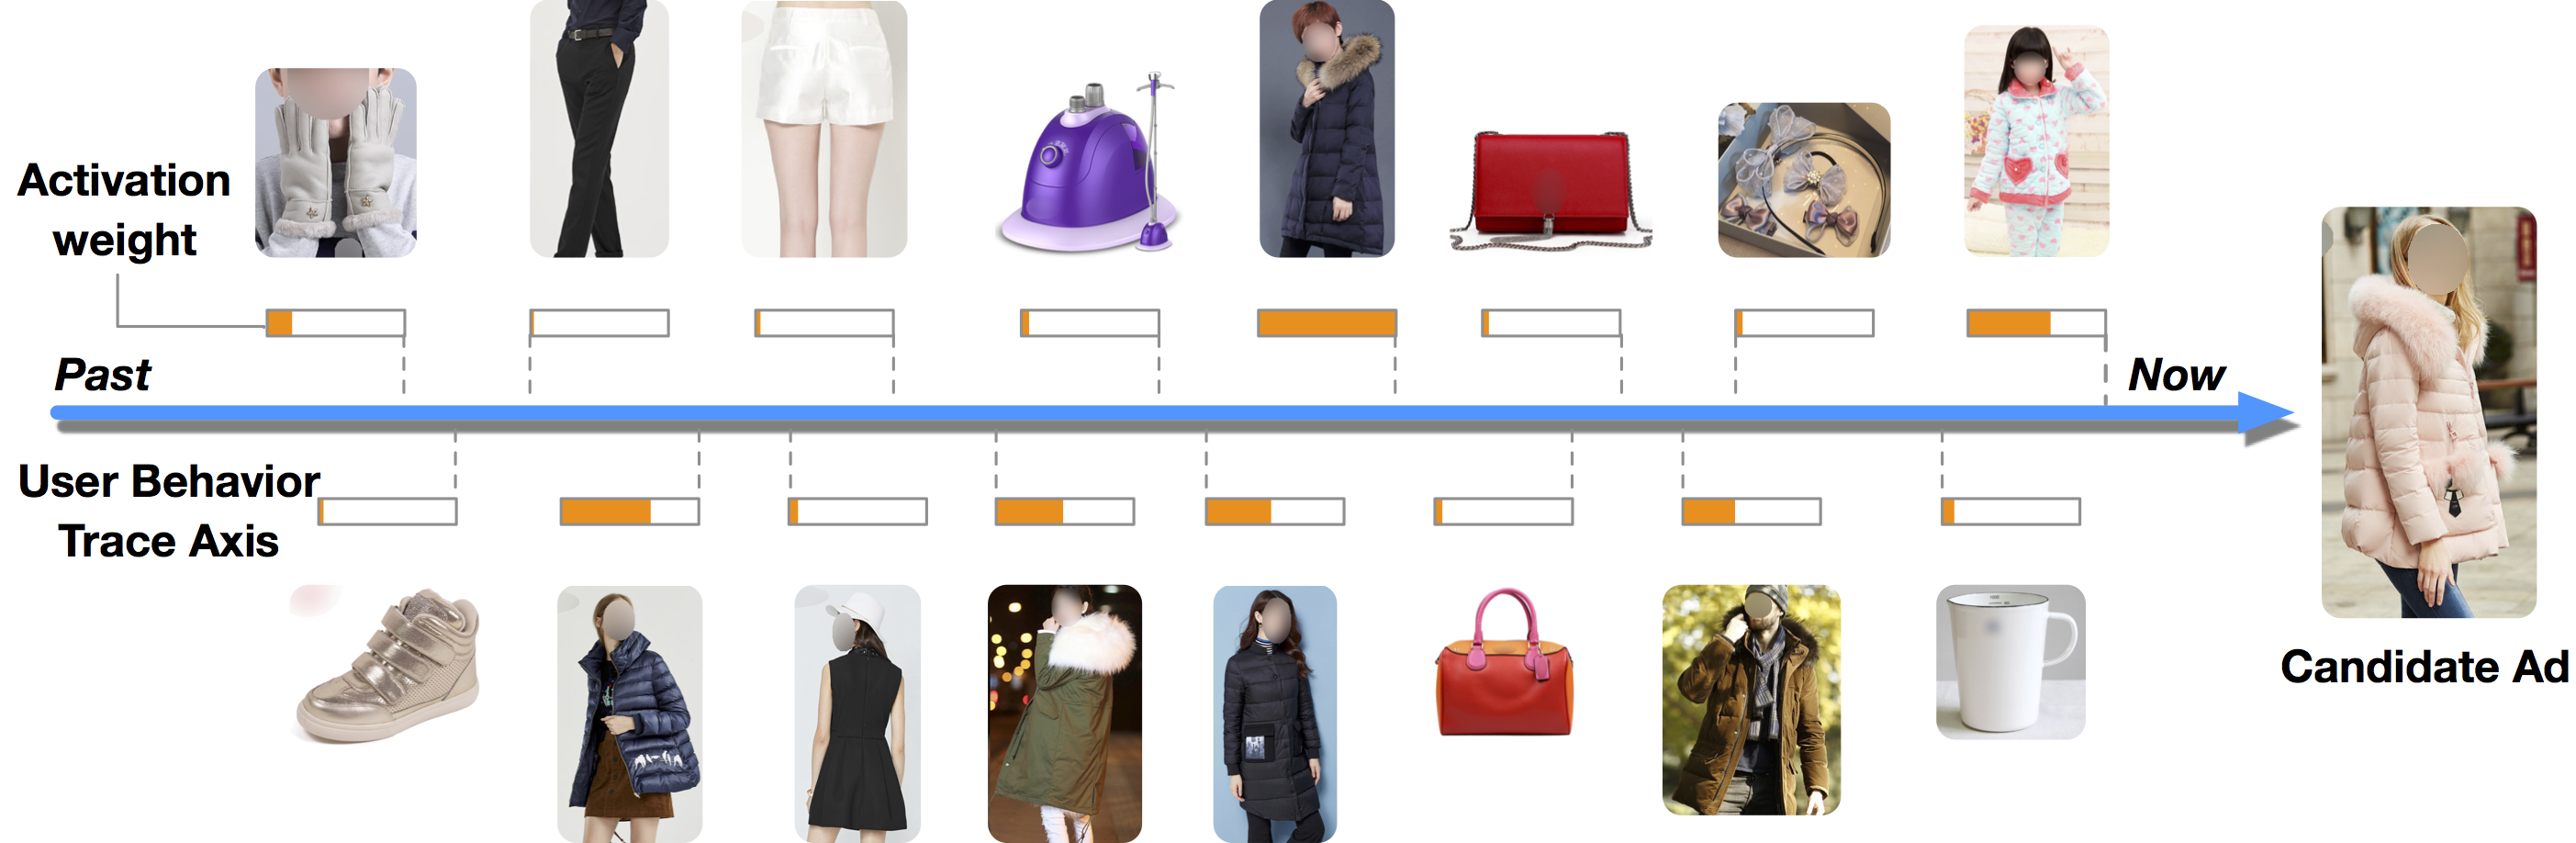
\includegraphics[height=2.5in, width=3.5in, keepaspectratio]{images/omni/attention_timeline_fix.png}
\caption{DIN 中自适应激活示意图。与候选广告高度相关的行为获得较高激活权重。}
\label{fig:att_case}
%\end{figure*}
\end{figure}


随后，我们可视化学习到的 embedding 向量。
以前文提到的年轻母亲为例，我们随机选择 9 个类别，如连衣裙、运动鞋、箱包等，并为每个类别选择 100 个商品作为她的候选广告。
图 \ref{fig:TDdiagram} 展示了 DIN 学习到的商品 embedding 向量的 t-SNE\cite{tsne} 可视化，其中形状相同的点对应同一类别。
可以看到，同一类别的商品几乎属于同一个簇，这清楚展示了 DIN embedding 的聚类性质。
此外，我们按预测值对表示候选广告的点着色。图 \ref{fig:TDdiagram} 也可看作这位母亲在 embedding 空间中对潜在候选项的兴趣密度分布热力图。它表明 DIN 能够在候选项的 embedding 空间中为某个用户形成多峰兴趣密度分布，从而捕获其多样化兴趣。




\begin{figure}[!t]
%\setlength{\belowcaptionskip}{-0.5cm}
\centering
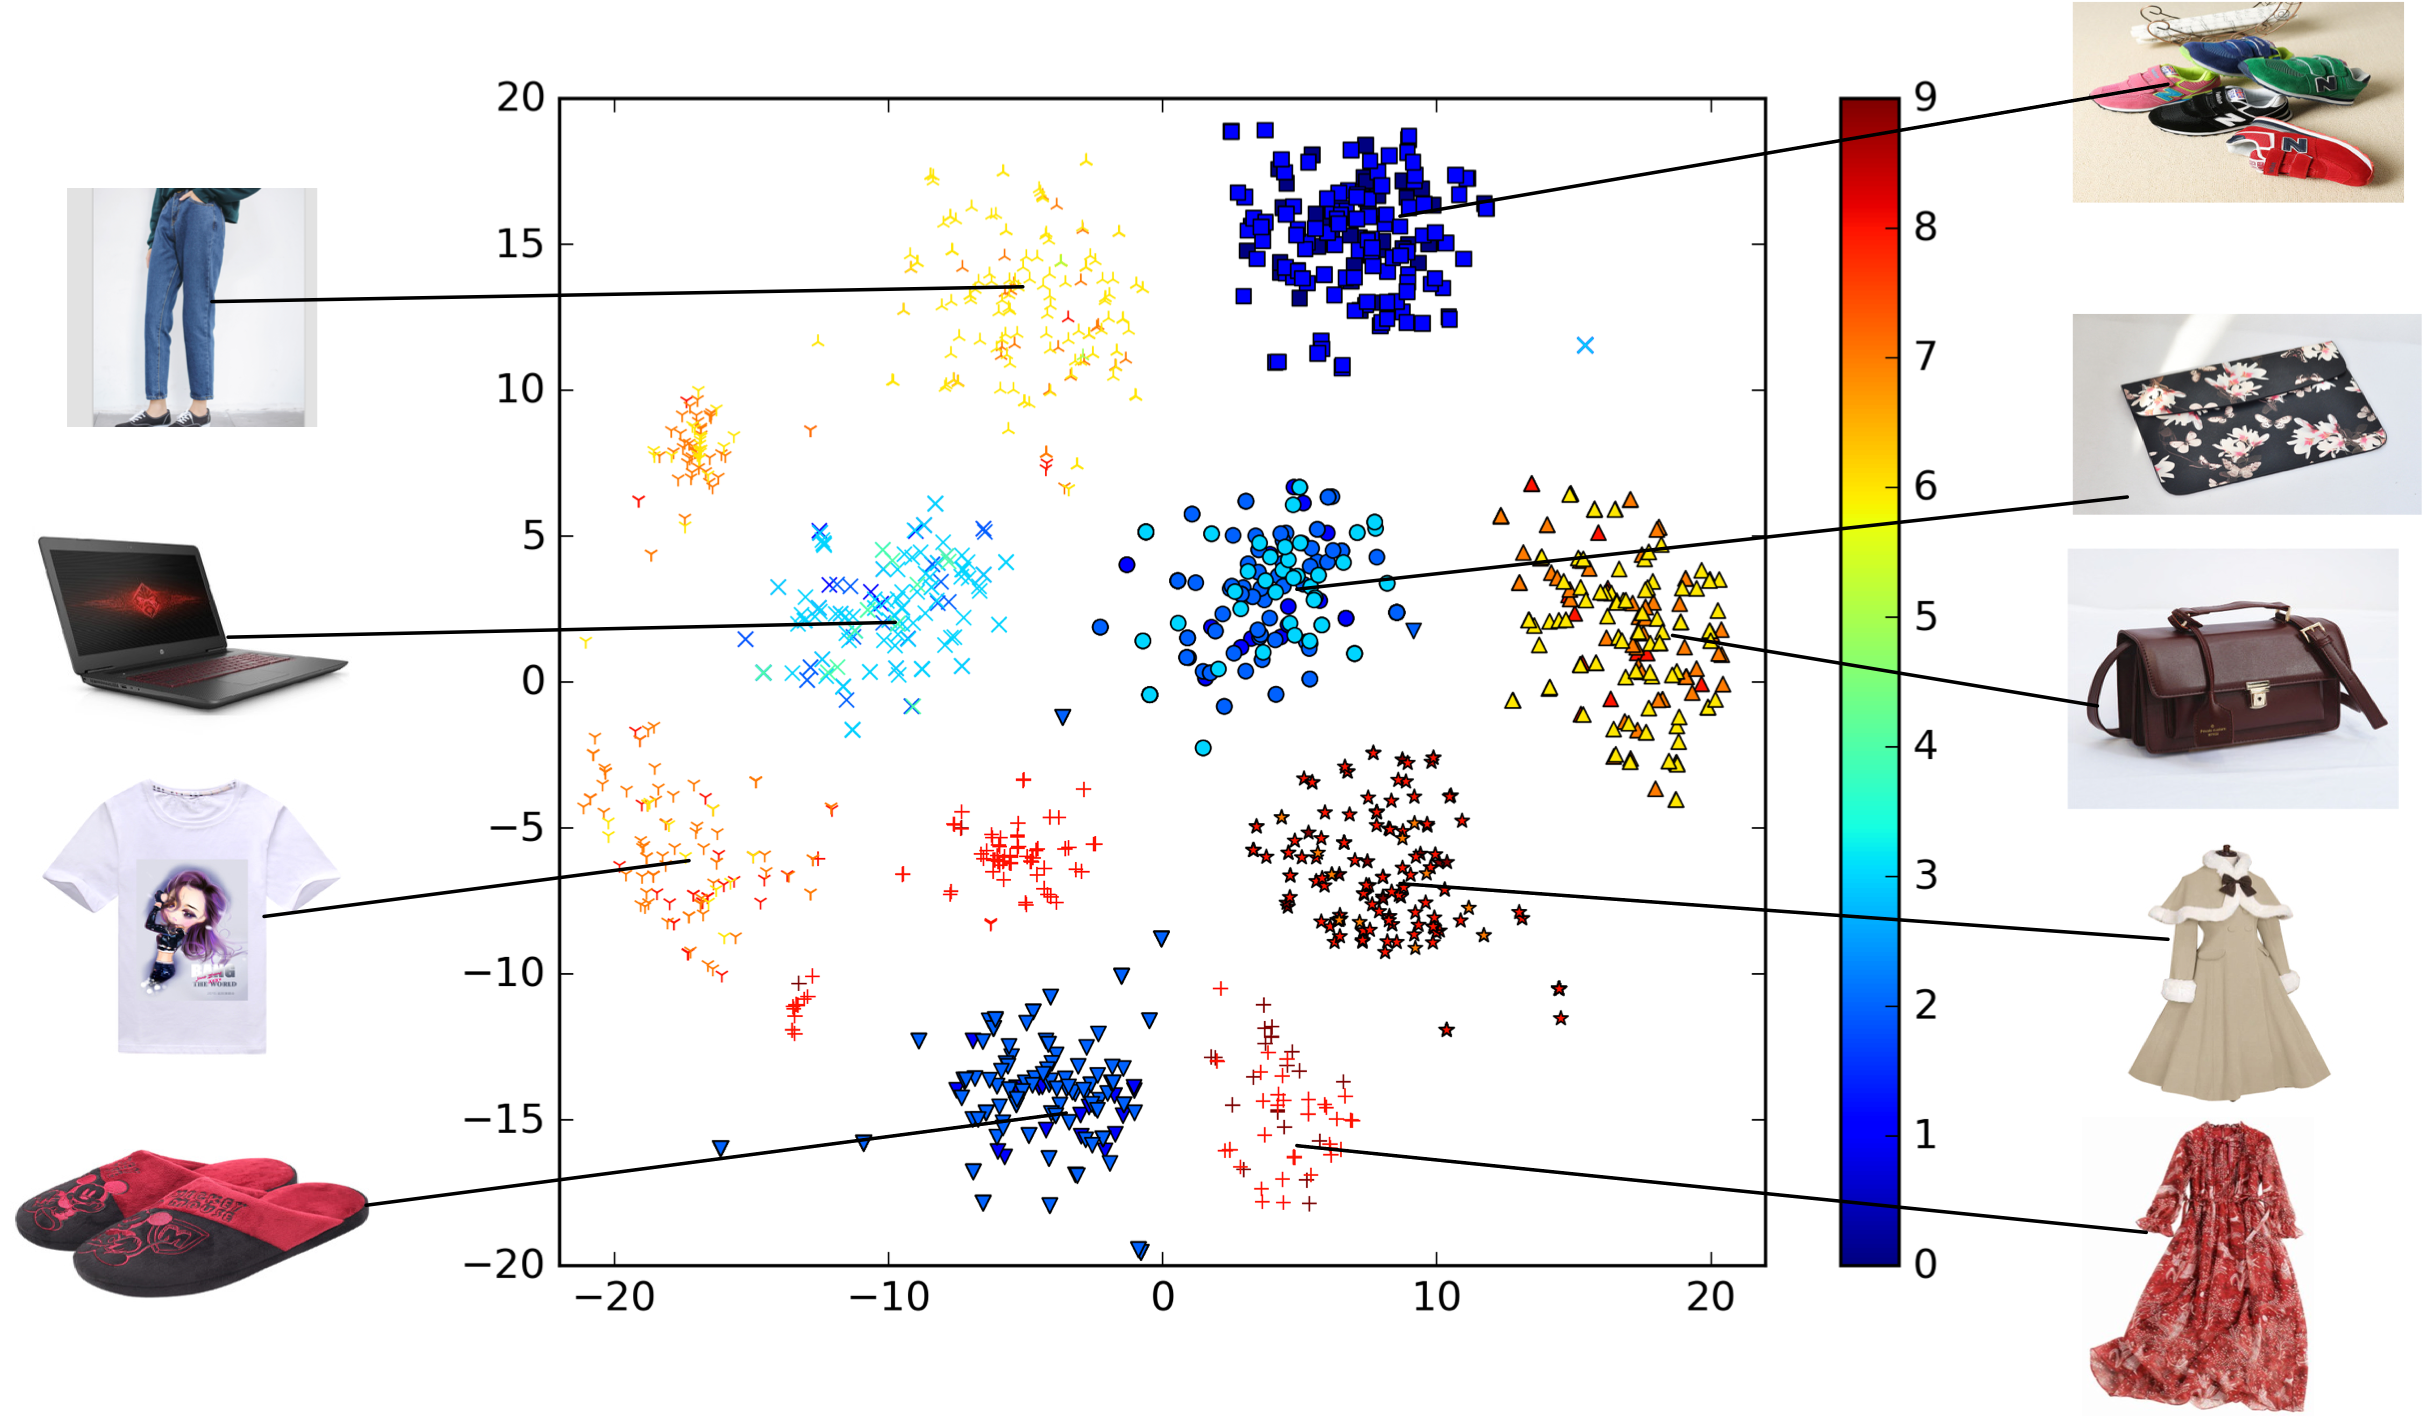
\includegraphics[height=2.5in, width=3.5in, keepaspectratio]{images/omni/TDdiagram.png}
\caption{DIN 中商品 embedding 的可视化。点的形状表示商品类别，点的颜色对应 CTR 预测值。}
\label{fig:TDdiagram}
\end{figure}



%Besides, we color the points that represent candidate ads by the prediction value. 
%Hot(red) points get higher CTR than cold(blue) ones.
%The red points appear in more than one clusters.
%Different categories of goods appearing the her historical behaviors are colored hot(red), which get higher CTR than those random candidates with cold(blue) color.  
%This demonstrates that DIN is able to capture diverse interests of a certain user, by forming a multimodal probability distribution of user interests in the embedding space.
